\documentclass[progress]{cmpreport}

\usepackage{rotating}
\usepackage{subfloat}
\usepackage{color}
\usepackage{pdfpages}
\usepackage{graphicx}
\usepackage[title,titletoc,toc]{appendix}
\usepackage{hyperref}
\usepackage{soul}

\title{Agri Robot Mapping and Pathing Progress Report}
\author{Toby Towler}
\registration{100395626}
\supervisor{Edwin Ren}
\ccode{CMP-6013Y}

\summary{This document provides an overview of my 12-week progress working on the "Agri Robot" project. I have been working on the pathing and mapping sections}


\begin{document}

\maketitle

\section{Introduction}
This "Agri Robot" was created by several masters students in a previous year,
I am working in a team to continue its development into a fully functioning product.
The robot is designed to function as an automated lawnmower, taking in a virtual map and mowing the entire area efficiently and accurately.
The robot will use an RTK chip to determine its location, as well as wheel odometry.
It will be able to detect its surroundings using a combination of LiDAR and camera technology, using these inputs to alter its path when necessary, for example if there is an animal in its path.
By the end, the robot should be able to know where it is, what's around it and where it's going next to a high degree of accuracy.
The final aim of this project is to have a finished, publishable and sellable product that could be used in the real world.

The tasks I have been working on so far are:
\begin{enumerate}
	\item {Random map generation}
	\item {Path generation}
	\item {Map generation from an aerial image}
\end{enumerate}

My motivation for this project is to make it run as fast and efficiently as possible, on the lowest specification hardware possible.
The algorithms produced during this project should be efficient in terms of both memory and processing power while still completing the task to an acceptable standard.
In a real world business context this would mean the production cost could be lowered, allowing either a lower selling price or higher profits.



\section{Progress}
\subsection{Mapping}
It is important to be able to test the robot's coverage of an area with many shapes of field to ensure it always works on any given area.
So there must be a way to generate maps to test all steps of the process on
Firstly, I had to build an algorithm to generate maps to represent fields. The maps are made up of the outline of the main field,
and a series of "holes" these would be trees or telegraph poles in real life, areas in the field that must be avoided by the robot.

My solution was the following:
\begin{enumerate}
	\item{Generate n random (x, y) points}
	\item{Select origin point with lowest y value}
	\item{Sort remaining points by polar angle to the origin point}
\end{enumerate}

This always produces a full polygon that never overlaps and can have any number of vertices where \hyperref[Mapping]{2}
For simplicity, I used a fixed origin of (0, 0) and generate points with positive x and y coordinates. Although the algorithm could be adapted to work with all random points.
The polar angle method comes from the Graham Scan for a convex hull \cite{geeksforgeeks2023}.
My algorithm is based on the first part of this idea.
This algorithm is repeated for the outline and the holes in the field, due to the varying number of vertices and random point generation, all polygons in the field can be different.


\subsubsection{Fields2Cover Mapping}
Fields2Cover (F2C) is a Complete Coverage Path Planning (CCPP) open source library, see next section.
I used this library primarily for CCPP, but it also has methods to generate \hyperref[F2CMapping]{fields of its own},
Which I used this for testing the F2C pathing solutions.

This method words by taking parameters for the area of the field and the number of vertices required.
There are no essential differences to using the F2C maps or my own algorithm as they both return a collection of 2-dimensional points meaning that the CCPP solution should be able to work with either map as input.

\subsection{Complete Coverage Path Planning}
Complete coverage path planning (CCPP) is the process of making a path for an object of width x to traverse an area while covering all points of the given area.
This is important for the agri robot as it needs to mow an entire area of grass leaving no area uncut to be a successful product.

My advisor showed me a paper tackling this problem with an open source library linked to it.
The library is called Fields2Cover (F2C) \cite{fields2cover2023github}, it is written in C++ and available as a C++ or python library.
At the beginning of trying to use the library, I had several compilation errors when trying to build from source.
I was able to fix the issues myself and then submit a GitHub pull request that was later approved, meaning I am now a contributor of this open source project.

After fixing these issues, I was able to use the library to generate CCPP solutions to inputs of any map.
There are several options to differ the final path making this a very flexible solution for a number of different applications
This library also allows easy configuration of the sizing, turning circle and velocities of the object to follow the path.

\subsection{Map Generation From An Aerial Image}
The idea of this task is that a drone could fly above an area and a suitable map be automatically generated with no user input.

As I have currently only just completed the CCPP problem, I have very little to show for this task.
I found some papers to read while doing previous research for mapping, reading these will be my next step as I try to find an appropriate algorithm.

\section{Progress Evaluation and Risk Analysis}
A big problem I have found so far during this project is finding algorithms or real world solutions that also apply to this problem.
Specifically for the CCPP aspect. There were very few open source algorithms or even discussions about a possible solution.
This was especially bad when the F2C source code did not compile, as this is the only way to use the library.
I spent a lot of time changing header files as well as C++ and Python build files in order to get it to finally work,
because of this it took me a lot longer to implement some features than I would have liked.

If the papers I have found so far do not prove very useful to this application,
This issue could repeat causing me to spend more time researching instead of adding features to the system.
Should this occur, I will analyze and talk to my team about if it would be better to move onto another feature where I could use my time more efficiently.
If the issue proves too hard to implement, I will also do this.

One concern I have about the future of this project is that additions to the code base will require libraries too big for the onboard memory of the Raspberry Pi,
or that some actions may be too complex for the processor to handle in real time.
If this does happen, I will need to change the way that my solution is implemented or change pre-existing parts of the code base to allow for greater consumption.



\newpage
\begin{appendix}
	\section{Appendix: 2.1 Mapping}

	\label{Mapping}
	\begin{figure}[H]
		\centering
		\begin{minipage}[b]{0.45\textwidth}
			\centering
			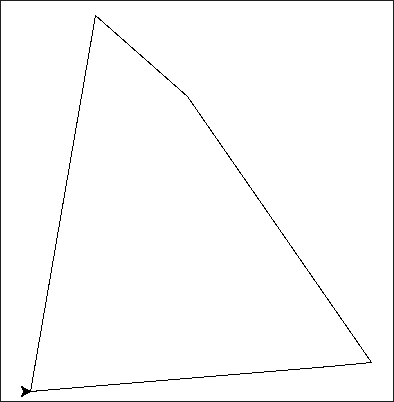
\includegraphics[width=\textwidth]{images/FirstMappingSmall.jpg}
			\caption{Polar angle method with 4 vertices}
		\end{minipage}
		\hfill
		\begin{minipage}[b]{0.45\textwidth}
			\centering
			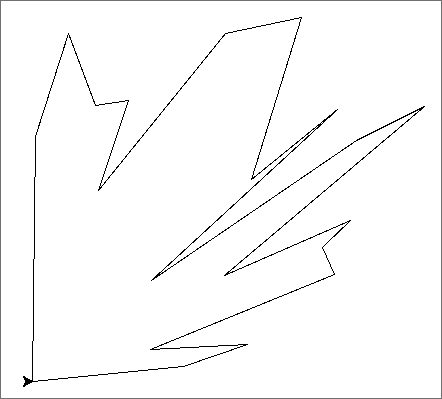
\includegraphics[width=\textwidth]{images/FirstMappingLarge.jpg}
			\caption{Polar angle method with 20 vertices}
		\end{minipage}
		\vspace{1em}

		\begin{minipage}[b]{0.45\textwidth}
			\centering
			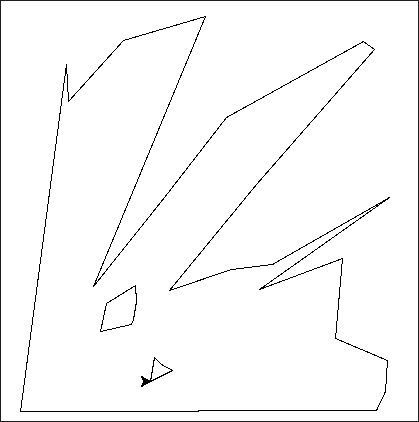
\includegraphics[width=\textwidth]{images/FirstMappingLargeHoles.jpg}
			\caption{Polar angle method with 2 holes}
		\end{minipage}
		\hfill

	\end{figure}

	\section{Appendix: 2.2 F2C Mapping}
	\label{F2CMapping}
	Note: Fields2Cover has its own drawing function which is used here

	\begin{figure}[H]
		\centering
		\begin{minipage}[b]{0.75\textwidth}
			\centering
			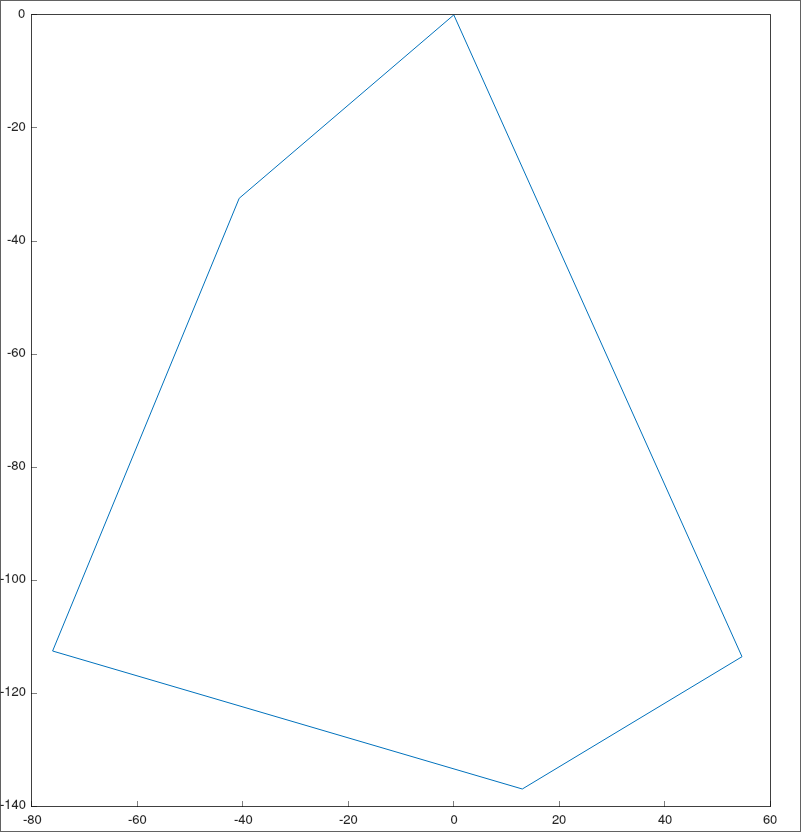
\includegraphics[width=\textwidth]{images/f2cMappingRandom.jpg}
			\caption{F2C randomly generated field with area 1e5 and 5 vertices}
		\end{minipage}

		\hfill
		\vspace{1em}

		\begin{minipage}[b]{0.75\textwidth}
			\centering
			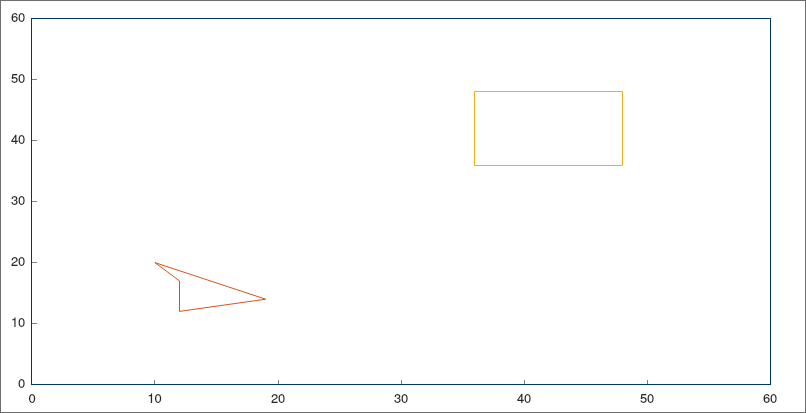
\includegraphics[width=\textwidth]{images/f2cMappingHoles.jpg}
			\caption{F2C field plotted with 2 holes}
		\end{minipage}

		\hfill

	\end{figure}
\end{appendix}

% \bibliographystyle{apalike}
\bibliography{ProgressReport}

\end{document}
